\section[Applications to Smooth Manifolds]{Applications to Smooth Manifolds: Non-Immersions and Cobordism}\lecture{08.01.24}
We will now discuss some applications of the preceding material in geometric topology.
In particular, we will see that smooth manifolds come with canonical vector bundles so that the Stiefel-Whitney classes become invariants of the manifold, and that the homotopy groups of $\Th(\gamma_\R^n)$ have geometric interpretations in terms of cobordism classes of smooth manifolds.

To start out, we recall (or learn anew) the following notions:
\begin{definition}
	Let $U \subseteq \R^m$ be open.
	A function $f\colon U \to Y \subseteq \R^n$ is \strong{smooth}\index{smooth function}\index{smooth map|see {smooth function}} if it is arbitrarily often differentiable.

	If $X \subseteq \R^m$ is any subset, then a function $f\colon X \to Y \subseteq \R^n$ is called \strong{smooth}\index{smooth function} if for every $x \in X$ there exists an open $x \in U \subseteq \R^m$ and a \strong{smooth extension}\index{smooth extension} of $f$ to $U$, i.e. a smooth function (in the previous sense) $\tilde{f}\colon U \to \R^n$ such that $\tilde{f}|_{U \cap X} = f|_{U \cap X}$.
\end{definition}
\begin{lemma}
	The composite of smooth maps is smooth.
\end{lemma}
\begin{proof}
	Omitted.
\end{proof}
\begin{definition}
	A function $f\colon X \to Y$ with $X \subseteq \R^m$, $Y \subseteq \R^n$ is a \strong{diffeomorphism}\index{diffeomorphism} if it is a smooth bijection with smooth inverse. 
	
	A subset $M \subseteq \R^m$ is a \strong{smooth manifold}\index{smooth manifold} of dimension $n$ if for all $x \in M$ there exists an open neighborhood $x \in U \subseteq M$ which is diffeomorphic to an open subset of $\R^n$.
\end{definition}
\begin{example}
	\leavevmode
	\begin{itemize}
		\item Any open subset of $\R^n$ is a smooth manifold.
		\item $S^n \subseteq \R^{n + 1}$ is a smooth manifold:
			For each $i = 1, \ldots, n + 1$ the open subsets 
			\begin{align*}
				U^+_i &\coloneq \{(x_1, \ldots, x_{n + 1}) \in S^n \mid x_i > 0 \} \\
				U^-_i &\coloneq \{(x_1, \ldots, x_{n + 1}) \in S^n \mid x_i < 0 \} 
			\end{align*}
			are diffeomorphic to the open disk $\mathring{D}^n$ via the projections
			\begin{align*}
				U^\pm_i &\to \mathring{D}^n \\
				(x_1, \ldots, x_{n + 1}) &\mapsto (x_1, \ldots, x_{i - 1}, x_{i + 1}, \ldots, x_{n + 1})
			\end{align*}
	\end{itemize}
\end{example}
\begin{remark}
	One can also define \enquote{abstract} smooth manifolds as second countable paracompact spaces $M$ equipped with addtional data in a variety of ways, for instance via equivalence classes of smooth atlases (cf. \cite[Ch. 1]{lee_introduction_2012}).
	One way is to specify for every open subset $U$ of $M$ a subset $F(U) \subseteq C^0(U, \R)$ of the ring of continuous functions on $U$ sucht that 
	\begin{enumerate}
		\item $F$ is a \emph{sheaf}\index{sheaf}, meaning that
			\begin{itemize}
				\item if $V \subseteq U$ is open and $f \in F(U)$, then $f|_V \in F(V)$, and 
				\item for every $x \in M$ there exists an open $U \ni x$ such that $(U, F|_U)$ is isomorphic to the sheaf $(\R^n, C^\infty({{-}}, \R))$ of smooth functions on $\R^n$.
			\end{itemize}
			A function $f\colon M \to N$ is then \strong{smooth}\index{smooth function} if $g \circ f \in F_M(f^{-1}(U))$ for all $U \subseteq N$ open and $g \in F_N(U)$.
	\end{enumerate}
\end{remark}
If $M \subseteq \R^m$ is a smooth submanifold, then (tautologically) defining $F(U) \coloneq \{f\colon U \to \R \text{ smooth}\}$ for all open $U \subseteq M$ defines a smooth structure on $M$ in this abstract sense.
Moreover, a map between submanifolds $f\colon M \to N$ is smooth if and only if it is smooth in the abstract sense. 
Hence, submanifolds of euclidean space form a full subcategory of abstract manifolds.
In fact, the categories are equivalent by the following result:
\begin{theorem}[Whitney embedding theorem]\footnote{(from me) A weaker lower bound of $\R^{2n + 1}$ can relatively easily be obtained from Sard's theorem, see e.g. \cite[Theorem 6.15]{lee_introduction_2012} (once one has established the equivalence of the definition via sheaves of smooth functions and via smooth atlases of smooth manifolds briefly mentioned above, which is not difficult). The proof of the stronger bound uses transversality and the Whitney trick, see for instance \cite{whitney_self-intersections_1944}.}\index{Whitney embedding theorem}
	Every abstract $n$-dimensional smooth manifold is diffeomorphic to a submanifold of $\R^{2n}$.
\end{theorem}
Let $M \subseteq \R^m$ be an $n$-dimensional manifold and $x \in M$ a point.
We define the \strong{tangent space}\index{tangent space}
\begin{equation*}
	\Tang_x M \coloneq D f_0(\R^n) \subseteq \R^m
\end{equation*}
where $f\colon V \xto{\isom} U \ni x$, $V \subseteq \R^n$ open is a choice of local parametrization such that $f(0) = x$ and $D f_0\colon \R^n \to \R^m$ is the derivative at $0 \in V$.
\begin{lemma}
	$\Tang_x M$ is independent of the choice of local parametrization.
\end{lemma}
\begin{proof}
	Omitted, see \cite[Section 1]{milnor_characteristic_1974}.
\end{proof}
\begin{definition}
	Let $M \subseteq \R^m$ be a smooth $n$-manifold.
	We define the \strong{tangent bundle}\index{tangent bundle} $\tau_M\colon \Tang M \to M$ with total space $\Tang M \coloneq \{(x, v) \in M \times \R^m \mid v \in \Tang_x M\}$ to be the projection $\tau_M(x, v) \coloneq x$.
\end{definition}
\begin{lemma}
	\leavevmode
	\begin{enumerate}
		\item This defines an $n$-dimensional $\R$-vector bundle over $M$ where we make each fibre carry the vector space structure on $\Tang_x M$.
		\item Moreover, every smooth map $f\colon M \to N$ between manifolds induces a bundle map defined via $d f_x(v) \coloneq \Tang f(x, v) \coloneq (f(x), D \tilde{f}_x(v))$ called its \strong{derivative}\index{derivative} or its \strong{differential}\index{differential|see {derivative}} where $\tilde{f}$ is a local extension of $f$ around $x$ to a smooth map on an open subset of $\R^m$.
	\end{enumerate}
\end{lemma}
\begin{proof}
	\leavevmode
	\begin{enumerate}
		\item Let $\varphi\colon V \xto{\isom} U$ be a local parametrization.
			Then
			\begin{align*}
				U \times \R^n &\to \Tang M|_U \\
				(y, v) &\mapsto \big(y, D_{\varphi^{-1}(y)}(v)\big)
			\end{align*}
			is an isomorphism.
		\item We omit the proof that this is independent of the extension $\tilde{f}$.
			\qedhere
	\end{enumerate}
\end{proof}
\begin{definition}
	Let $M \subseteq \R^m$ be an $n$-dimensional smooth manifold.
	Its \strong{normal bundle}\index{normal bundle} $\nu_{M, \R^m}$ is defined as the orthogonal complement of the tangent bundle $\tau_M$ viewed as a subbundle of the trivial bundle $M \times \R^m$, i.e. its total space is given by 
	\begin{equation*}
		\Nu_{M, \R^m} \coloneq \{(x, v) \in M \times \R^m \mid v \in (\Tang_x M)^\perp\}
	\end{equation*}

	More generally, let $i\colon M \to N \subseteq \R^m$ be an \strong{immersion}\index{immersion}, i.e. a smooth map such that the derivative $d i_x\colon \Tang_x M \to \Tang_{i(x)} N$ is injective for all $x \in M$.
	Then the normal bundle $\nu_i$ has total space
	\begin{equation*}
		\Nu_i \coloneq \big\{(x, v) \in M \times \R^m \mid v \in T_{i(x)} N,\ v \perp d i_x(\Tang_x M)\big\}
	\end{equation*}
	with $\nu_i((x, v)) = x$ the projection so that $i^* \tau_N \isom \tau_M \dsum \nu_i$, i.e. $\nu_i$ is the orthogonal complement of $\tau_M$ inside $i^* \tau_N$.
\end{definition}
Note that immersions are local but not necessarily global embeddings:
For instance, the map 
\begin{center}
	\tikzsetnextfilename{smthmflds_circle_immersion}
	\begin{tikzpicture}[thick]
		\draw (0, 0) circle[radius = 1.7];
		\begin{scope}[yscale = .75, xscale = 1.2, xshift = 4cm]
			\draw plot[smooth cycle, tension = 1, xshift = 6] coordinates {(-1, 2) (1, 2) (-.7, 0) (1, -2) (-1, -2) (.7, 0)};
		\end{scope}
		\draw[commutative diagrams/every arrow] (2.2, 0) -- +(1.5, 0);
	\end{tikzpicture}
\end{center}
is an immersion.
Also, $\RP^2$ and the Klein bottle can be immersed into $\R^3$ but not embedded.
\begin{example}
	We have $\Tang_x S^n = \{v \in \R^n \mid v \perp x\} = \langle x \rangle^\perp$.

	It suffices to show this for $x = (0, \ldots, 0, 1)$ since for any other $x' \in S^n$ there exists an isometry $A \in \Ort(n + 1)$ such that $A x = x'$ which sends $\langle x \rangle^\perp$ to $\langle x' \rangle^\perp$ whilst mapping $\Tang_x S^n$ isomorphically onto $\Tang_{x'} S^n$ since it is an orthogonal transformation.

	For the north pole $x = (0, \ldots, 0, 1)$ we use the parametrization
	\begin{align*}
		f\colon \mathring{D}^n &\to U \coloneq U^+_{n + 1} = \{(y_1, \ldots, y_{n + 1}) \in S^n \mid y_{n + 1} > 0\} \\
		(y_1, \ldots, y_n) &\mapsto \big(y_1, \ldots, y_n, \sqrt{1 - |y|^2}\big)
	\end{align*}
	with derivative
	\begin{equation*}
		\pgfset{nicematrix/cell-node/.append style = {outer sep = -4pt}}
		D f_y = {\renewcommand{\arraystretch}{1.6}\begin{pmatrix}
			I_n \\
			\frac{y}{\sqrt{1 - |y|^2}}
		\end{pmatrix}} =
		\begin{pNiceMatrix}[columns-width = auto]
			1   &       & \Block{2-3}<\Large>{0} \\
			&   1   &        &      &       \\
			&       &   1    &      &       \\
			\Block{2-3}<\Large>{0} &       &       & \Ddots    &   \\
			&       &       &      &   1   \\
			\frac{y_1}{\sqrt{1 - |y|^2}} & \Cdots & & & \frac{y_n}{\sqrt{1 - |y|^2}}
		\end{pNiceMatrix}
	\end{equation*}
	Hence, $D f_0(\R^n) = \R^n \times \{0\} = \langle x \rangle^\perp$.
	The normal bundle is thus given by $\Nu_{S^n, \R^{n + 1}} = \{(x, v) \in S^n \times \R^{n + 1} \mid v \in \langle x \rangle\}$ and is therefore isomorphic to the trivial line bundle via
	\begin{align*}
		S^n \times \R &\xto{\isom} \Nu_{S^n, \R^{n + 1}} \\
		(x, \lambda) &\mapsto (x, \lambda x)
	\end{align*}
	so $\tau_{S^n} \dsum \nu_{S^n, \R^{n + 1}} \isom \tau_{S^n} \dsum \epsilon \isom \epsilon^{n + 1}$ and $\omega(\tau_{S^n}) = \omega(\tau_{S^n} \dsum \epsilon) = \omega(\epsilon^{n + 1}) = 1$ for the total Stiefel-Whitney class.
	Nevertheless, one can show that $\tau_{S^n}$ is trivializable if and only if $n = 1$, 3, or 7.
	This is closely related to the Hopf invariant 1 problem.
\end{example}

We now want to discuss $\RP^n$, which first we have to turn into a smooth manifold.
This we can do in two ways:
\begin{enumerate}
	\item Declare a function $f\colon U \to \R$ defined on a open subset $U \subseteq \RP^n$ to be smooth if the composite $p^{-1}(U) \xto{p} U \xto{f} \R$ where $p\colon S^n \to \RP^n$ is the 2-fold covering map is smooth; or
	\item Identify $\RP^n$ with a subspace of $\R^{(n + 1) \times (n + 1)} \isom M_{n + 1}(\R)$ via the map $A_{-}\colon L = \langle x \rangle \mapsto A_L \coloneq \frac{1}{|x|^2}(x_i x_j)_{i, j}$, or, in words, the map that sends a line in $\R^{n + 1}$ to the orthogonal projection onto that line.
		This map is clearly injective, and the composite
		\begin{equation*}
			\begin{tikzcd}[row sep = -.3ex, /tikz/column 1/.append style = {anchor = base east}]
				\tilde{g}\colon S^n
						\ar[r, "p"]
					& \RP^n
						\ar[r, "A_{-}"]
					& M_{n + 1}(\R)
				\\
				x
						\ar[rr, mapsto]
					& & (x_i x_j)_{i, j}
			\end{tikzcd}
		\end{equation*}
		is smooth with smooth inverse:
		For any line $L$, pick a unit vector $e_i$ not contained in $L^\perp$.
		Then the map $A_{L'} \mapsto A_{L'}(e_i) / |A_L(e_i)|$ is a local smooth inverse to $A_{-}$ around $L$.
		Hence, the image of $A_{-}$ is a smooth manifold and $p\colon S^n \to \RP^n \isom \img(A_{-})$ is a local diffeomorphism.
		In particular, $d p_x\colon \Tang_x S^n = \langle x \rangle^\perp \to \Tang_{\langle x \rangle} \RP^n$ is an isomorphism for all $x \in S^n$.
		Since any line $L \in \RP^n$ has exactly two preimages in $S^n$, which are of the form $x$, $-x$, and these satisfy $\Tang_x S^n = \langle x \rangle^\perp = \langle -x \rangle^\perp = \Tang_{-x} S^n$, this identifies $\Tang_L \RP^n$ with $L^\perp$.
		But this is misleading:
		The two isomorphisms
		\begin{align*}
			d p_x\colon \langle x \rangle^\perp &\xto{\isom} \Tang_{\langle x \rangle} \RP^n \\
			d p_{-x}\colon \langle -x \rangle^\perp &\xto{\isom} \Tang_{\langle -x \rangle} \RP^n
		\end{align*}
		satisfy $d p_x = -d p_{-x}$ since the antipode $\alpha\colon S^n \to S^n$ sends $x \to -x$, has derivative $d \alpha = -I_n$, and satisfies $p \circ \alpha = p$.
		To encode this, we instead identify $\Tang \RP^n$ with the set of all pairs
		\begin{equation*}
			\{(x, v), (-x, -v) \mid v \perp x\} \subseteq S^n \times \R^n
		\end{equation*}
		which is by construction independent of the choice of generator $x \in L$ under the antipodal map.
		The fibre over a line $L$ identifies with the set of homomorphisms $\gamma\colon L \to L^\perp$ via $\gamma \mapsto \{(x_1, \gamma(x_1)), (x_2, \gamma(x_2))\}$ where $x_1$, $x_2$ are the two unit length generators of $L$.
		We therefore obtain:
\end{enumerate}
\begin{corollary}
	The tangent bundle $\Tang \RP^n$ is isomorphic to the \emph{hom-bundle}\index{hom-bundle} $\Hom\big(\gamma_\R^{1, n}, (\gamma_\R^{1, n})^\perp\big)$.
\end{corollary}
\lecture{12.01.24}
\begin{remark}
	If $M$ is a smooth $n$-manifold and $i\colon M \to \RP^m$ an immersion, then there is a continuous map
	\begin{align*}
		M &\to \Gr_n(\R^m) \\
		x &\mapsto d i_x(\Tang_x M)
	\end{align*}
	which is covered by the bundle map (known as the \strong{Gauss map}\index{Gauss map})
	\begin{align*}
		\Tang M &\to E\big(\gamma_\R^{n, m}\big) \\
		(x, v) &\mapsto (d i_x(\Tang_x M), d i_x(v))
	\end{align*}
	Hence, the composite $M \to \Gr_n(\R^m) \incl \Gr_n^\R$ classifies the tangent bundle $\tau_M$ under the bijection
	\begin{equation*}
		\Vect_\R^n(M) \isom \big[M, \Gr_n^\R\big]
	\end{equation*}
	The same construction works for the normal bundle $\nu_i$ of $i$, which is classified by the map
	\begin{align*}
		M &\to \Gr_{m - n}(\R^m)\;\big(\incl \Gr_{m - n}^\R\big) \\
		x &\mapsto d i_x(\Tang_x M)^\perp
	\end{align*}
\end{remark}

Now let $i\colon M \to \R^m$ be an immersion of a smooth $n$-manifold $M$ into euclidean space.
We can consider the total Stiefel-Whitney class of the tangent bundle
\begin{equation*}
	\omega(\tau_M) = 1 + \omega_1(\tau_M) + \ldots \in H^\pi(M; \F_2)
\end{equation*}
Let $1 + \overline{\omega_1}(\tau_M) + \ldots \eqcolon \overline{\omega}(\tau_M) \coloneq \omega(\tau_M)^{-1} \in H^\pi(M; \F_2)$ be its inverse.
\begin{proposition}\label{prop:vanishingomegainverse}
	We have $\overline{\omega}_j(\tau_M) = 0$ for $j > m - n$.
\end{proposition}
\begin{proof}
	Let $\nu_i$ be the normal bundle for the immersion $i$.
	Then $\tau_M \dsum \nu_i = \epsilon^n$ and hence $\omega(\nu_i) = \omega(\tau_M)^{-1} = \overline{\omega}(\tau_M)$.
	Since $\nu_i$ is $(m - n)$-dimensional, the claim follows from the dimensionality axiom of the Stiefel-Whitney classes.
\end{proof}

We now want to study immersions of projective spaces, for which we need to understand $\overline{\omega}(\tau_{\RP^n})$.
\begin{theorem}
	There is an isomorphism
	\begin{equation*}
		\tau_{\RP^n} \dsum \epsilon \isom \bigdsum^{n + 1} \gamma_\R^{1, n + 1}
	\end{equation*}
	Hence,
	\begin{equation*}
		\omega(\tau_{\RP^n}) = \omega(\tau_{\RP^n} \dsum \epsilon) = (1 + u)^{n + 1} = \sum_{j = 0}^n \binom{n + 1}{j} u^j
	\end{equation*}
	since $u^{n + 1} = 0 \in H^*(\RP^n; \F_2)$.
\end{theorem}
\begin{proof}
	The line bundle $\Hom(\gamma_\R^{1, n + 1}, \gamma_\R^{1, n + 1})$ over $\RP^n$ is trivializable since the identity map gives a canonical non-zero element in each fibre.
	Hence, we compute
	\begin{align*}
		\Hom(\gamma_\R^{1, n + 1}, (\gamma_\R^{1, n + 1})^\perp) \dsum \epsilon &\isom \Hom(\gamma_\R^{1, n + 1}, (\gamma_\R^{1, n + 1})^\perp) \dsum \Hom(\gamma_\R^{1, n + 1}, \gamma_\R^{1, n + 1}) \\
																				&\isom \Hom(\gamma_\R^{1, n + 1}, \underbrace{(\gamma_\R^{1, n + 1})^\perp \dsum \gamma_\R^{1, n + 1}}_{\isom \epsilon^{n + 1}}) \\
																				&\isom \Hom(\gamma_\R^{1, n + 1}, \epsilon^{n + 1}) \\
																				&\isom \bigdsum^{n + 1} \Hom(\gamma_\R^{1, n + 1}, \epsilon)
	\end{align*}
	Finally, we have $\Hom(\gamma_\R^{1, n + 1}, \epsilon) \isom \gamma_\R^{1, n + 1}$ since $\gamma_\R^{1, n + 1}$ admits a euclidean metric that allows us to canonically identify each fibre with its dual.
\end{proof}
\begin{corollary}
	If $\tau_{\RP^n}$ is trivializable, then $n + 1$ must be a power of 2.
\end{corollary}
\begin{proof}
	If $n + 1 = 2^r m$ with $m > 1$ odd, then
	\begin{align*}
		\omega(\tau_{\RP^n}) &= (1 + u)^{2^r m} \\
							 &= (1 + u^{2^r})^m \\
							 &= 1 + \underbrace{m u^{2^r}}_{= u^{2^r} \neq 0} + \text{ higher order terms}
	\end{align*}
	contradicting triviality of the Stiefel-Whitney classes of a trivial bundle.
\end{proof}
Regarding non-immersions of $\RP^n$, we focus on the case $n = 2^k$ where the results are sharpest.
In this case, we have $\omega(\tau_{\RP^n}) = (1 + u)^{2^k + 1} = (1 + u)(1 + u^{2k}) = 1 + u + u^{2^k}$ and hence $\overline{\omega}(\tau_{\RP^n}) = 1 + u + u^2 + \cdots + u^{2^k - 1}$ since
\begin{align*}
	(1 + u + u^{2^k})(1 + u + u^2 + \cdots + u^{2^k - 1}) &= (1 + u)(1 + u + u^2 + \cdots + u^{2^k - 1} + u^{2^k}) \\
														  &= 1 + u^{2^k} + u^{2^k} \\
														  &= 1
\end{align*}
\begin{corollary}
	If $\RP^{2^k}$ immerses into $\R^m$, then $m \geq 2^k + (2^k - 1)$.
\end{corollary}
\begin{proof}
	This follows from the preceding computation and proposition \ref{prop:vanishingomegainverse}.
\end{proof}
Generally, we have
\begin{theorem}[Whitney]\index{Whitney immersion theorem}
	Every smooth $n$-manifold ($n \geq 1$) immerses into $\R^{2n - 1}$.
\end{theorem}
Hence our bound for $\RP^{2^k}$ is optimal, but in general the bounds for immersions of $\RP^m$ into euclidean space obtained by this method are not.
In fact, the lowest possible dimensions are generally not know to this date.
Better bounds can nevertheless be obtained via characteristic classes of generalized cohomology theories.

For general $m$, let $\alpha(m)$ be the number of set bits in its binary expansion, so that $m = \sum_{i = 1}^{\alpha(m)} 2^{n_i}$ with $n_1 < \ldots < n_{\alpha(m)}$.
Let $M = \RP^{2^{n_1}} \times \cdots \times \RP^{2^{n_{\alpha(m)}}}$.
Then $\overline{\omega}(\tau_M) = \overline{\omega}\big(\tau_{\RP^{n_1}}\big) \times \cdots \times \overline{\omega}\big(\tau_{\RP^{n_{\alpha(m)}}}\big)$ with highest non-trivial term $u^{2^{n_1} - 1} \times \cdots \times u^{2^{n_{\alpha(m)}} - 1}$ in degree $m - \alpha(m)$.
The \emph{immersion conjecure}\index{immersion conjecture} states that if $N$ is any $m$-manifold, then $N$ immerses into $\R^{2m - \alpha(m)}$.
A proof of this was claimed by Ralph L. Cohen in his 1985 paper \cite{cohen_immersion_1985}, but its correctness is controversial.

We now turn to the final topic of the course:
\subsection{Bordism}
\begin{note}
	In this section, all manifolds will be assumed smooth.
\end{note}
We write $\H^n$ for the \strong{upper half-plane}\index{upper half-plane} $\H^n \coloneq \{(x_1, \ldots, x_n) \mid x_1 > 0\} \subset \R^n$ of $\R^n$.
\begin{definition}
	A subset $X \subset \R^n$ is a \strong{$n$-manifold with boundary}\index{manifold!with boundary} if for each $x \in X$ there is a neighborhood $U \subseteq X$ which is diffeomorphic to an open subset of $\H^n$.
	Given such an $X$, we say that $x \in X$ is an \strong{interior point}\index{interior point} of $X$ if it has a neighborhood diffeomorphic to an open subset of $\R^n$ (which is true if and only if $H_n(X, X \setminus \{x\}; \Z) \isom \Z$).

	The interior points $\mathring{X}$ form an open subset of $X$ which is an $n$-dimensional (non-compact) manifold (without boundary), whereas the \strong{boundary}\index{boundary!of a manifold} $\del X$ of $X$, i.e. the space of all non-interior points, forms a $(n - 1)$-manifold (again without boundary).
\end{definition}
For brevity's sake, we will take \enquote{compact manifold} to mean \enquote{compact manifold with or without boundary} and \enquote{\strong{closed}\index{closed manifold} manifold} to mean \enquote{compact manifold without boundary.}

We can then define two variants of bordism, one internal and one external:
\begin{definition}\index{cobordant manifolds}\index{bordism}
	\leavevmode
	\begin{itemize}
		\item Two closed $n$-manifolds $M$, $M'$ in $\R^m$ are called \strong{cobordant in $\R^m$} if there exists a $(n + 1)$-dimensional compact manifold with boundary $N \subseteq \R^m \times [0, 1]$ such that
			\begin{enumerate}
				\item there exists an $\epsilon > 0$ such that $N \cap (\R^m \times [0, \epsilon)) = M \times [0, \epsilon)$ and $N \cap (\R^m \times (1 - \epsilon, 1]) = M' \times (1 - \epsilon, 1]$, and
				\item the boundary of $N$ is $\del N = N \cap (\R^m \times \{0, 1\}) = M \times \{0\} \sqcup M' \times \{1\}$.
					% TODO picture
			\end{enumerate}
		\item Two closed $n$-manifolds $M$, $M'$ (in possibly different-dimensional euclidean spaces) are called \strong{cobordant} if there exists a compact $(n + 1)$-dimensional manifold with boundary $N$ such that $\del N$ is diffeomorphic to $M \sqcup M'$.
	\end{itemize}
\end{definition}

Note that there is no collar assumption in the abstract definition since differential topology provides us with the following theorem:
\begin{theorem}[Collar neighborhood theorem]\index{collar neighborhood theorem}\label{thm:collarnbhd}
	If $N$ is a manifold with boundary, then there exists an open neighborhood of $\del N$ in $N$ which is diffeomorphic to $\del N \times [0, 1)$.
\end{theorem}
For a proof see \cite[Theorem 9.25]{lee_introduction_2012}.
\begin{lemma}
	Both bordism in $\R^m$ and abstract bordism are equivalence relations.
\end{lemma}
\begin{proof}
	We only treat bordism in $\R^m$; the abstract case is also not hard.
	\begin{itemize}
		\item \strong{Reflexivity:} $N = M \times [0, 1] \subseteq \R^m \times [0, 1]$ is a bordism from $M$ to itself.
		\item \strong{Symmetry:} If $N \subseteq \R^m \times [0, 1]$ is a bordism from $M$ to $M'$, then $\overline{N} \coloneq \{(x, t) \mid (x, 1 - t) \in N\}$ is a bordism from $M'$ to $M$.
		\item \strong{Transitivity:} If $N \subseteq \R^m \times [0, 1]$ is a bordism from $M$ to $M'$ and $N' \subseteq \R^m \times [1, 2]$ is a bordism from $M'$ to $M''$, then $N'' \coloneq N \cup N' \subseteq \R^m \times [0, 2]$ is a bordism from $M$ to $M''$:
			Indeed, by the collar assumption, $N''$ agrees with $M' \times (1 - \epsilon, 1 + \epsilon)$ around $\R^m \times \{1\}$ and hence forms a smooth manifold with boundary.
			% TODO picture
			\qedhere
	\end{itemize}
\end{proof}
We write 
\begin{equation*}
	\Bord_n^{(m)} \coloneq \{M \mid M \text{ closed } n \text{-manifold in } \R^m\} /\,\text{bordism in } \R^m
\end{equation*}
and 
\begin{equation*}
	\Bord_n \coloneq \{M \mid M \text{ closed } n \text{-manifold}\} /\,\text{bordism}
\end{equation*}
for the sets of equivalence classes.

We have stabilization maps $\Bord_n^{(m)} \to \Bord_n^{(m + 1)}$ and maps $\Bord_n^{(m)} \to \Bord_n$ that forget the embedding in euclidean space.
The Whitney embedding theorem for manifolds with boundary\index{Whitney embedding theorem!for manifolds with boundary} implies that the map $\colim_{m \in \N} \Bord_n^{(m)} \to \Bord_n$ is a bijection, i.e. bordism in infinite-dimensional euclidean space $\R^\infty$ is equivalent to abstract cobordism.

We next note that $\Bord_n^{(m)}$ and $\Bord_n$ both come with additional structure:
Let $M, M' \subseteq \R^m$ be closed $n$-manifolds.
Then, by replacing $M'$ with cobordant manifold if necessary, we can assume that $M$ and $M'$ are disjoint. For instance, the translate $(M' + v)$ for any $v \in \R^m$ is cobordant to $M'$ via $N = \{(m' + \alpha(t)v, t) \mid m' \in M', t \in [0, 1]\}$ where $\alpha\colon [0, 1] \to \R$ is a smooth function satisfying 
\begin{equation*}
	\alpha(t) = \begin{cases}
		0 & t < 1 / 4 \\
		1 & t > 3 / 4
	\end{cases}
\end{equation*}
The disjoint union is then again a closed $n$-manifold.
\begin{lemma}
	The bordism class of $M \sqcup M'$ only depends on the bordism classes of $M$ and $M'$.
	The operation
	\begin{align*}
		\Bord_n^{(m)} \times \Bord_n^{(m)} &\to \Bord_n^{(m)} \\
		([M], [M']) &\mapsto [M \sqcup M']
	\end{align*}
	turns $\Bord_n^{(m)}$ into a 2-torsion abelian group with neutral element $[\emptyset]$\footnote{(from me) It is customary to consider the empty set as a compact manifold without boundary of every dimension in this context.}.
\end{lemma}
\begin{proof}
	Clear.
\end{proof}
Similarly $\Bord_n$ becomes a 2-torsion abelian group via disjoint union.
Moreover, we have
\begin{lemma}
	Given $[M] \in \Bord_n$, $[M'] \in \Bord_{n'}$, the product
	\begin{equation*}
		[M] \times [M'] \coloneq [M \times M'] \in \Bord_{n + n'}
	\end{equation*}
	is well-defined, associative and commutative.
	Thus, $\Bord_* \coloneq \bigdsum_{n \in \N} \Bord_n$ forms a graded, commutative $\F_2$-algebra.
\end{lemma}
\begin{proof}
	If $N$ is a bordism from $M_1$ to $M_2$, then $N \times M'$ is a bordism from $M_1 \times M'$ to $M_2 \times M'$ and likewise in the other variable.
	Associativity and commutativity follow directly from the respective properties of the product of spaces.
\end{proof}
\lecture{15.01.24}
Our main goal here is to understand $\Bord_*$.
We study this ring via the so-called \emph{Stiefel-Whitney numbers}\index{Stiefel-Whitney numbers} defined as follows:

Let $M$ be a closed $n$-manifold.
There is then a fundamental class $\mu_M \in H_n(M; \F_2)$ and we obtain a homomorphism
\begin{equation*}
		\begin{tikzcd}[row sep = -.2ex]
		H^n(M; \F_2)
				\ar[r, "\isom"]
			& \Hom(H_n(M; \F_2), \F_2)
				\ar[r, "\ev_{\mu_M}"]
			& \F_2
		\\
		x 
				\ar[rr, mapsto]
			& & \langle x, \mu_M \rangle
	\end{tikzcd}
\end{equation*}
Further, let $r_1, \ldots, r_n \in \N$ be such that $r_1 + 2 r_2 + \ldots + n r_n = n$.
Then the product $\omega_1(\tau_M)^{r_1} \cdots \omega_n(\tau_M)^{r_n}$ lies in $H^n(M; \F_2)$ and we obtain a number
\begin{equation*}
	\big\langle \omega_1(\tau_M)^{r_1} \cdots \omega_n(\tau_M)^{r_n}, \mu_M \big\rangle \in \F_2
\end{equation*}
called the \strong{Stiefel-Whitney number}\index{Stiefel-Whitney numbers} of $M$ associated to the sequence $(r_1, \ldots, r_n)$ and denoted $\omega_1^{r_1} \cdots \omega_n^{r_n}[M] \in \F_2$.
\begin{example}
	Let $M = \RP^n$.
	We distinguish two cases:
	\begin{enumerate}
		\item $n$ is even.
			Then $\omega_n\big(\tau_{\RP^n}\big) = (n + 1) u^n \neq 0$ so $\omega_n[\RP^n] \neq 0$.
			Generally speaking, the Stiefel-Whitney numbers in this case are products of binomial coefficients which again turn out to be particularly simple if $n = 2^k$ for some $k \geq 1$:
			We have
			\begin{equation*}
				\omega\big(\tau_{\RP^{2^k}}\big) = 1 + u + u^{2^k}
			\end{equation*}
			hence $\omega_1^{2^k}\big[\RP^{2^k}\big] \neq 0$, but $\omega_1^{r_1} \cdots \omega_n^{r_n}\big[\RP^{2^k}\big] = 0$ for all monomials except $\omega_1^{2^k}$ and $\omega_{2^k}$.
		\item $n = 2k - 1$ is odd.
			Then $\omega\big(\tau_{\RP^n}\big) = (1 + u)^{2k} = (1 + u^2)^k$ and hence $\omega_i\big(\tau_{\RP^n}\big) = 0$ if $i$ is odd.
			If $r_1 + 2 r_2 + \ldots + n r_n = 2k - 1$, then at least one $r_i$ with $i$ odd has to be non-zero, hence $\omega_1^{r_1} \cdots \omega_n^{r_n}[\RP^n] = 0$ for all such sequence $(r_1, \ldots, r_n)$.
	\end{enumerate}
\end{example}

The Stiefel-Whitney numbers are bordism invariants:
\begin{theorem}
	If a closed $n$-manifold $M$ is the boundary of a compact $(n + 1)$-manifold, then all Stiefel-Whitney numbers of $M$ are zero.
\end{theorem}
\begin{proof}
	There is a relative fundamental class $\mu_N \in H_{n + 1}(N, M; \F_2)$ which maps to $\mu_M$ under the boundary map $\del\colon H_{n + 1}(N, M; \F_2) \to H_n(M; \F_2)$.
	For any $x \in H^n(M; \F_2)$ we then have
	\begin{equation*}
		\big\langle x, \mu_M \big\rangle = \big\langle x, \del \mu_M \big\rangle = \big\langle \delta x, \mu_N \big\rangle
	\end{equation*}
	where $\delta\colon H^n(M; \F_2) \to H^{n + 1}(N, M; \F_2)$ is the coboundary map by the compatibility of the evaluation pairing $\langle {{-}}, {{-}} \rangle$ with (co)boundary operators.
	From the collar neighborhood theorem (\ref{thm:collarnbhd}), it follows that a neighborhood of $M$ in $N$ is diffeomorphic to $M \times [0, \epsilon)$.
	Hence, we get to consider a \enquote{shifted} copy of $M$ as sitting inside the interior of $N$ with trivial normal line bundle\footnote{One can alternatively work with the tangent space of the boundary directly without using collar neighborhoods, but this requires some more work to set up.}.
	It follows that $(\tau_N)|_M \isom \tau_M \dsum \epsilon$ and hence $i^*(\omega(\tau_{\mathring{N}})) = \omega(\tau_M)$ where $i\colon M \incl N$ is the inclusion.
	Hence, each $\omega_i(\tau_M)$ lies in the image of $i^*\colon H^i(N; \F_2) \to H^i(M; \F_2)$ and therefore so does every monomial $\omega_1^{r_1}(\tau_M) \cdots \omega_n^{r_n}(\tau_M) \in H^n(M; \F_2)$.
	By exactness, every such monomial thus maps to zero under $\delta\colon H^n(M; \F_2) \to H^{n + 1}(N, M; \F_2)$ and we obtain
	\begin{align*}
		\omega_1^{r_1} \cdots \omega_n^{r_n}[M] &= \big\langle \omega_1^{r_1}(\tau_M) \cdots \omega_n^{r_n}(\tau_M), \mu_M \big\rangle \\ 
												&= \big\langle \underbrace{\delta(\omega_1^{r_1}(\tau_M) \cdots \omega_n^{r_n}(\tau_M))}_{= 0}, \mu_N \big\rangle \\
												&= 0 
												\qedhere
	\end{align*}
\end{proof}
\begin{corollary}
	If $n$ is even, then $\RP^n$ is not the boundary of a compact $(n + 1)$-manifold.
\end{corollary}
\begin{corollary}
	If $M$ is cobordant to $M'$, then
	\begin{equation*}
		\omega_1^{r_1} \cdots \omega_n^{r_n}[M] = \omega_1^{r_1} \cdots \omega_n^{r_n}[M']
	\end{equation*}
	for all sequences $(r_1, \ldots, r_n)$ with $r_1 + 2 r_2 + \ldots + n r_n = n$.
\end{corollary}
\begin{proof}
	Since $M$ is cobordant to $M'$, the disjoint union $M \sqcup M'$ is the boundary of a compact $(n + 1)$-manifold, so all Stiefel-Whitney numbers of $M \sqcup M'$ are zero.
	We thus have
	\begin{equation*}
		0 = \omega_1^{r_1} \cdots \omega_n^{r_n}[M \sqcup M'] = \omega_1^{r_1} \cdots \omega_n^{r_n}[M] + \omega_1^{r_1} \cdots \omega_n^{r_n}[M']
	\end{equation*}
	since $\mu_{M \sqcup M'} = \mu_M + \mu_{M'} \in H^n(M; \F_2) \dsum H^n(M'; \F_2) \isom H^n(M \sqcup M'; \F_2)$ and the Stiefel-Whitney classes are computed component-wise, so we conclude that both summands must be equal for all monomials.
\end{proof}
\begin{example}
	We have
	\begin{align*}
		\omega\big(\tau_{\RP^2 \times \RP^2}\big) &= \omega\big(\tau_{\RP^2}\big) \times \omega\big(\tau_{\RP^2}\big) \\
												  &= (1 + u_1 + u_1^2) \times (1 + u_2 + u_2^2) \\
												  &= 1 + \underbrace{u_1 \times 1 + 1 \times u_2}_{= \omega_1} + \underbrace{u_1 \times u_2 + u_1^2 \times 1 + 1 \times u_2^2}_{= \omega_2} \\ 
												  &\qquad\quad + \underbrace{u_1 \times u_2^2 + u_1^2 \times u_2}_{= \omega_3} + \underbrace{u_1^2 \times u_2^2}_{= \omega_4}
	\end{align*}
	where $u_1$ and $u_2$ are the generators of $H^*(\RP^2; \F_2)$ in the respective factors.
	There are Stiefel-Whitney numbers associated to the following sequences:
	\begin{itemize}
		\item $(4, 0, 0 ,0)$: $\omega_1^4 = 0$.
		\item $(2, 1, 0 ,0)$: $\omega_1^2 \omega_2 = u_1^2 \times u_2^2 + u_1^2 \times u_2^2 = 0 $.
		\item $(1, 0, 1 ,0)$: $\omega_1 \omega_3 = u_1^2 \times u_2^2 + u_1^2 \times u_2^2 = 0 $.
		\item $(0, 2, 0 ,0)$: $\omega_2^2 = u_1^2 \times u_2^2 \neq 0 $.
		\item $(0, 0, 0 ,1)$: $\omega_4 = u_1^2 \times u_2^2 \neq 0 $.
	\end{itemize}
	so
	\begin{align*}
		\omega_1^4[\RP^2 \times \RP^2] &= 0 \\
		\omega_1^2 \omega_2[\RP^2 \times \RP^2] &= 0 \\
		\omega_1 \omega_3[\RP^2 \times \RP^2] &= 0 \\
		\omega_2^2[\RP^2 \times \RP^2] &= 1 \\
		\omega_4[\RP^2 \times \RP^2] &= 1
	\end{align*}
	We have already seen that the only non-zero Stiefel-Whitney numbers of $\RP^4$ are $\omega_1^4[\RP^4]$ and $\omega_4[\RP^4]$.
	It follows that $\RP^4$, $\RP^2 \times \RP^2$, and $\RP^4 \sqcup \RP^2 \times \RP^2$ represent pairwise different, non-trivial cobordism classes and $\Bord_4$ is at least 2-dimensional as an $\F_2$-vector space.
\end{example}
We can also consider the 4-manifold $\CP^2$ which can be equipped with a smooth structure in an analogous manner to real projective space, and by the same computation satisfies $\tau_{\CP^2} \isom \Hom_\C(\gamma_\C^{1, 3}, (\gamma_\C^{1, 3})^\perp)$, or more precisely, the real bundle underlying this complex bundle.
Using the same argument as in the real case, we can compute its Chern-classes via
\begin{align*}
	c\big(\Hom_\C(\gamma_\C^{1, 3}, \big(\gamma_\C^{1, 3}\big)^\perp)\big) &= c\big(\Hom_\C\big(\gamma_\C^{1, 3}, \epsilon_\C^3\big)\big) \\
														   				   &= c\big(\Hom_\C\big(\gamma_\C^{1, 3}, \epsilon_\C\big)\big)^3
\end{align*}
As $\Hom_\C\big(\gamma_\C^{1, 3}, \epsilon_\C\big)$ is the tensor inverse of $\gamma_\C^{1, 3}$, we find that
\begin{equation*}
	c_1\big(\Hom_\C\big(\gamma_\C^{1, 3}, \epsilon\big)\big) = -c_1\big(\gamma_\C^{1, 3}\big) = -u \in \Z[u] / u^3 \isom H^*(\CP^2; \Z)
\end{equation*}
Hence, $c\big(\Hom_\C\big(\gamma_\C^{1, 3}, \big(\gamma_\C^{1, 3}\big)^\perp\big)\big) = (1 - u)^3 = 1 - 3u + 3u^2$.
To understand the Stiefel-Whitney classes of the underlying real bundle, we have the following lemma:
\begin{lemma}
	Let $\xi$ be a complex vector bundle over a paracompact base $B$ and $\xi_\R$ its underlying real bundle.
	Then:
	\begin{enumerate}
		\item\label{lma:swofcomplexbundle:1} $\omega_i(\xi_\R) = 0$ if $i$ is odd.
		\item\label{lma:swofcomplexbundle:2} $\omega_{2i}(\xi_\R)$ is the modulo 2 reduction of $c_i \in H^{2i}(B; \Z)$.
	\end{enumerate}
\end{lemma}
In other words, the modulo 2 reduction of $c(\xi_\R)$ equals $\omega(\xi_\R)$.
\begin{proof}
	It suffices to show this for the universal case $\xi = \gamma_\C^n$, $n > 0$.
	Since $H^*\big(\Gr_n^\C; \F_2\big) \isom \F_2[\bar{c}_1, \ldots, \bar{c}_n]$ with $\bar{c}_i$ the modulo 2 reduction of $c_i$ is concentrated in even degrees, property \ref{lma:swofcomplexbundle:1} follows.

	For property \ref{lma:swofcomplexbundle:2}, the claim follows by induction on $n$ for all $i < n$ by the commutative square
	\begin{equation*}
		\tikzsetnextfilename{smthmdflds_commsquare}
		\begin{tikzpicture}[
			% setup some helpers to declutter the matrix head below
			gray column/.style args = {#1}{
				column #1/.append style = {
					knowngray
				},
			},
			column separators/.style args = {#1/#2}{
				column #1/.append style = {
					column sep = #2,
				},
			},
			row separators/.style args = {#1/#2}{
				row #1/.append style = {
					row sep = #2,
				},
			},
			commutative diagrams/.cd, 
			every diagram, 
			sep = large]
			\matrix[
				matrix of math nodes, 
				name = m, 
				commutative diagrams/every matrix,
				commutative diagrams/every cell,
				gray column/.list = {2, 3},
				% not the ideal way to to this but whatevs
				column separators/.list = {1/-2.2em, 2/5.7em, 3/-2.5em},
				row separators/.list = {1/-.6ex, 2/3.7ex, 3/-.6ex}] {
					H^{2i}\big(\Gr_n^\C; \Z\big) 	& & & H^{2i}\big(\Gr_{n - 1}^\C; \Z\big) 	\\
						& c_i 	& c_i 			\\
						& 		& \omega_{2i} 	\\
					H^{2i}\big(\Gr_n^\C; \F_2\big) 	& & & H^{2i}\big(\Gr_{n - 1}^\C; \F_2\big) 	\\
			};
			\draw[commutative diagrams/.cd, every arrow, every label]
				(m-1-1) edge["$\isom$"] (m-1-4)
						edge (m-4-1)
				(m-1-4) edge (m-4-4)
				(m-4-1) edge["$\isom$"] (m-4-4);
			\draw[commutative diagrams/.cd, every arrow, every label, mapsto, knowngray]
				(m-2-2) edge (m-2-3)
				(m-2-3) edge (m-3-3);
		\end{tikzpicture}
	\end{equation*}
	The remaining class $c_n \in H^{2n}\big(\Gr_n^\C; \Z\big)$ is defined as the Euler class for the sphere bundle $S(\gamma_\C^n) \to \Gr_n^\C$ (recall theorem \ref{thm:cohomology_gr_C}).
	Since the orientation class reduces to the unique $\F_2$-orientation class, it follows that the reduction of the integral Euler class is the $\F_2$-Euler class.
	As we saw that the Euler class for the $\F_2$-orientation gives the top Stiefel-Whitney class $\omega_{2n}$, this completes the proof.
\end{proof}
We conclude that $\omega\big(\tau_{\CP^2}\big) = 1 + u + u^2 = 1 + \omega_2 + \omega_4 \in H^*(\CP^2; \F_2) \isom \F_2[u] / u^3$.
Any Stiefel-Whitney numbers associated to a sequence containing an odd number must hence be trivial.
The remaining sequences are:
\begin{itemize}
	\item $(0, 2, 0, 0)$: $\omega_2^2 = u^2 \neq 0$, so $\omega_2^2[\CP^2] \neq 0$.
	\item $(0, 0, 0, 1)$: $\omega_4 = u^2 \neq 0$, so $\omega_4[\CP^2] \neq 0$.
\end{itemize}
Thus, the Stiefel-Whitney numbers of $\CP^2$ and $\RP^2 \times \RP^2$ agree, and in fact one can show that the two manifolds are cobordant.
Much more generally, René Thom proved the following: 
\edef\thomcitestring{Corollaire \uppercase\expandafter{\romannumeral 4\relax}.11 \& Théorème \uppercase\expandafter{\romannumeral 4\relax}.12}
\begin{theorem}[{\cite[\thomcitestring]{thom_quelques_1954}}]
	\leavevmode
	\begin{enumerate}
		\item Any two closed $n$-manifolds $M$ and $M'$ with identical Stiefel-Whitney numbers are cobordant.
		\item The cobordism ring $\Bord_*$ is isomorphic to a polynomial ring of the form $\F_2[x_i \mid i + 1 \text{ not a power of } 2]$ with $x_i$ of degree $i$.
	\end{enumerate}
\end{theorem}
\begin{remark}
	In particular we have:
	\begin{itemize}
		\item $\Bord_1 = 0$: Every closed 1-manifold is a boundary\footnote{(from me) Of course, the only such manifolds are finite disjoint unions of copies of $S^1$ by the classification of 1-manifolds, so this could easily be deduced by elementary means as well.}.
		\item $\Bord_2 \isom \F_2\{x_2\}$ is 1-dimensional over $\F_2$.
			Since we saw that $[\RP^2]$ is non-trivial, we must have $x_2 = [\RP^2]$.
		\item $\Bord_3 = 0$: Every closed 3-manifold is a boundary.
		\item $\Bord_4 \isom \F_2\{x_2^2, x_4\}$ is 2-dimensional over $\F_2$.
			We already saw that $[\RP^2 \times \RP^2]$ and $[\RP^4]$ are linearly independent, so they must form a basis and $x_4$ can be taken to be either $[\RP^4]$ or $[\RP^2 \times \RP^2]$.
	\end{itemize}
\end{remark}
\lecture{19.01.24}
\begin{remark}
	In general, $x_{2i}$ can be taken to be $[\RP^{2i}]$.
	The following possible choices for the $x_n$ where $n$ is odd were first given by Albrecht Dold in \cite{dold_erzeugende_1956}:
	Let $m, n \geq 0$ and set
	\begin{equation*}
		P(m, n) \coloneq (S^m \times \CP^n) / C_2
	\end{equation*}
	where $C_2$ acts on $P(m, n)$ by the antipode in the first coordinate and complex conjugation in the second, i.e. via $(x, y) \mapsto (-x, \bar{y})$.
	For example, we directly see that $P(m, 0) = \RP^m$ and $P(0, n) = \CP^n$.

	Since the $C_2$ action is free and smooth (and proper as $C_2$ is compact), $P(m, n)$ inherits the structure of a smooth manifold from $S^m \times \CP^n$ by the \emph{quotient manifold theorem}\index{quotient manifold theorem}, see for example \cite[Theorem 21.10]{lee_introduction_2012}.
	Dold shows that:
	\begin{enumerate}
		\item $H^*(P(m, n); \F_2) \isom \F_2[c, d] / (c^{m + 1}, d^{n + 1})$ with $|c| = 1$, $|d| = 2$.
			In fact, the Serre spectral sequence for the fibre sequence
			\begin{align*}
				\CP^n \to P(m, n) &\to \RP^m \\
				[(x, y)] &\mapsto [x]
			\end{align*}
			collapses on the $E_2$-page.
		\item $\Sq^1(d) = cd$.
		\item $\omega(\tau_{P(m, n)}) = (1 + c)^m (1 + c + d)^{n + 1}$.
		\item In Thom's theorem, one can take
			\begin{equation*}
				x_i = \begin{cases}
					[P(i, 0)] = [\RP^i] & i \text{ even} \\
					[P(2^r - 1, s 2^r)] & i \text{ odd}
				\end{cases}
			\end{equation*}
			where $i + 1 = 2^r (2s + 1)$.
	\end{enumerate}
\end{remark}

For the remainder of the course we will discuss the proof of Thom's theorem.
The first step is to interpret the groups $\Bord_n^{(m)}$ and $\Bord_n$ homotopy-theoretically using the \strong{Thom-Pontryagin construction}\index{Thom-Pontryagin construction}.

We will need to make use of the following concept from differential topology:
\begin{definition}
	Let $M \subseteq \R^n$ be a manifold with normal bundle $\nu_{M, \R^n}$.
	A \strong{tubular neighborhood}\index{tubular neighborhood} of $M$ is a smooth embedding $f\colon E(\nu_{M, \R^n}) \incl \R^n$ such that:
	\begin{enumerate}
		\item $f|_M = \id_M$ where $M$ is identified with the image of the zero-section of $\nu_{M, \R^n}$.
		\item $f(E(\nu_{M, \R^n}))$ is an open neighborhood of $M$ in $\R^n$.
	\end{enumerate}
\end{definition}
\begin{example}\label{ex:tubbynbdhsn}
	The map
	\begin{align*}
		f\colon E(\nu_{S^n, \R^{n + 1}}) &\to \R^{n + 1} \\
		(x, v) &\mapsto x + \frac{v}{3(1 + \lVert v \rVert)}
	\end{align*}
	is a tubular neighborhood of $S^n \subset \R^{n + 1}$.
\end{example}
\begin{figure}[ht]
	\centering
	\tikzsetnextfilename{smthmdflds_tubbynbhd_s_1}
	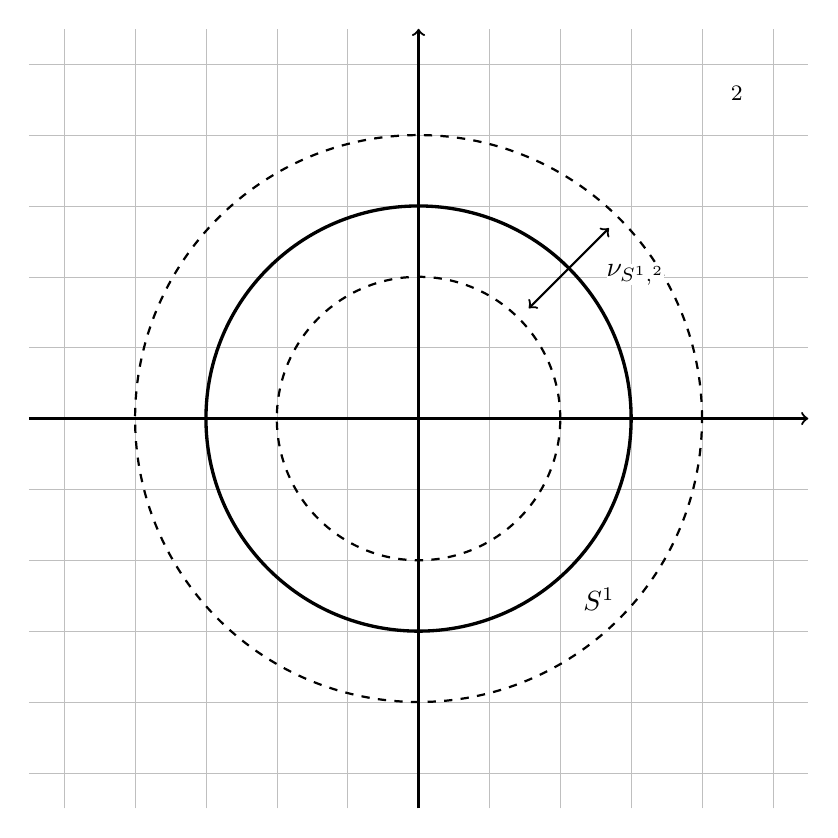
\begin{tikzpicture}[scale = .9, thick, every node/.style = {fill = white}]
		\draw[very thin, lightgray] (-5.5, -5.5) grid (5.5, 5.5);

		\draw[->] (-5.5, 0) -- (5.5, 0);
		\draw[->] (0, -5.5) -- (0, 5.5);

		\node[font = \large] at (4.5, 4.5) {$\R^2$};

		\draw[very thick] (0, 0) circle[radius = 3cm];
		\draw[dashed] 
			(0, 0) circle[radius = 2cm] 
			(0, 0) circle[radius = 4cm];

		\begin{scope}[rotate = -45]
			\draw[->] (0, 3) -- (0, 3.8);
			\draw[->] (0, 3) -- (0, 2.2);
			\node[inner sep = 0pt] at (.73, 3.6) {$\nu_{S^1, \R^2}$};
		\end{scope}


		\node[inner sep = 0pt] at (-45:3.6cm) {$S^1$};
	\end{tikzpicture}
	\caption{The tubular neighborhood from example \ref{ex:tubbynbdhsn} illustrated in the case $n = 1$.}
\end{figure}
\begin{theorem}[Tubular neighborhood theorem]\index{tubular neighborhood theorem}\label{thm:tubbynbhds}
	Every compact\footnote{(from me) This theorem holds more generally even for non-compact manifolds, cf. \cite[Theorem 6.24]{lee_introduction_2012}.} manifold $M \subseteq \R^n$ admits a tubular neighborhood.
\end{theorem}
\begin{proof}[Sketch of proof]
	As in example \ref{ex:tubbynbdhsn}, we define a map
	\begin{align*}
		f_\lambda\colon E(\nu_{M, \R^n}) &\to \R^n \\
		(x, v) &\mapsto x + \frac{v}{\lambda(1 + \lVert v\rVert)}
	\end{align*}
	The implicit function theorem implies that each $f_\lambda$ is an immersion on an open neighborhood of $M \subseteq E(\nu_{M, \R^n})$.
	The fact that $f_\lambda|_M = \id_M$ and compactness of $M$ then imply that for $\lambda \gg 0$ the map $f|_\lambda$ is an embedding.
\end{proof}
We now view $S^n = \R^n \cup \{\infty\}$ as pointed with basepoint $\infty$, and for a euclidean bundle $\xi\colon E \to B$ we equip $\Th(\xi) = D(\xi) / S(\xi)$ with the basepoint $[S(\xi)]$, the collapsed boundary of the disk bundle.

Let $M \subseteq \R^n$ be a closed $k$-dimensional submanifold with tubular neighborhood as constructed in the proof of theorem \ref{thm:tubbynbhds}.
Then we can define a continuous, pointed map
\begin{equation*}
	\Phi_M\colon S^n \to \Th(\gamma_\R^{n - k})
\end{equation*}
via the composite
\begin{equation*}
	\begin{tikzcd}[row sep = large]
		S^n 
				\ar[r, two heads]
			& S^n \big/ f\big(\mathring{D}(\nu_{M, \R^n})\big)^{\mathrm{C}}
			& f\big(D(\nu_{M, \R^n})\big) \big / f\big(S(\nu_{M, \R^n})\big)
				\ar[l, swap, "\isom"]
				\ar[from = 2-1, rounded corners, to path = {[pos = 1.1]
					-- ([xshift = -2ex] \tikztostart.west)
					|- ($(\tikzcdmatrixname-1-2)!0.5!(\tikzcdmatrixname-2-2)$) \tikztonodes
					-| ([xshift = 1em] \tikztotarget.east)
					-- (\tikztotarget)
				}, "f", "\isom"']
		\\
			\Th(\nu_{M, \R^n})
				\ar[r, "\Th(g)"]
			& \Th(\gamma_\R^{n - k, n})
				\ar[r, "(\R^n \incl \R^\infty)_*"]
			& \Th(\gamma_\R^{n - k})
	\end{tikzcd}
\end{equation*}
where $g\colon E(\nu_{M, \R^n}) \to E(\gamma_\R^{n - k, n})$ is the Gauss map of the normal bundle of $M$.
\begin{proposition}\label{prop:pontryaginthom}
	\leavevmode
	\begin{enumerate}
		\item If $M, M' \subseteq \R^n$ are cobordant, then $\Phi_M$ is based-homotopic to $\Phi_{M'}$.
		\item Let $n > 1$ and $M_1, M_2 \subseteq \R^n$ be two closed manifolds.
			Assume that $M_1 \subseteq \mathring{D}_1$, $M_2 \subseteq \mathring{D}_2$ with $D_1 \cap D_2 = \emptyset$ two disjoint closed disks.
			Then $\Phi_{M_1 \sqcup M_2}$ represents the sum of $[\Phi_{M_1}]$ and $[\Phi_{M_2}]$ in $\pi_n(\Th(\gamma_\R^{n - k}))$.
	\end{enumerate}
\end{proposition}
\begin{corollary}
	The map
	\begin{align*}
		\Phi\colon \Bord_k^{(n)} &\to \pi_n(\Th(\gamma_\R^{n - k})) \\
		[M] &\mapsto [\Phi_M]
	\end{align*}
	is a group homomorphism.
\end{corollary}
\begin{proof}[Proof of proposition \ref{prop:pontryaginthom}]
	Let $N \subseteq \R^n \times [0, 1]$ be a cobordism from $M$ to $M'$.
	We can extend $N$ slightly to include $M \times \{0\}$ and $M' \times \{1\}$ in its interior by adding on $M \times (-\delta, 0]$ and $M' \times [1, 1 + \delta)$ for some small $\delta > 0$.
	
	Let $f\colon E(\nu_{N, \R^n}) \to \R^n$ be a tubular neighborhood for $N$. 
	Noting that by construction we have $E(\nu_{N, \R^n})_x = E(\nu_{M, \R^n})_x \times \{0\}$ for all $x \in M$ and likewise for $M'$, the restrictions $f^{\mathring{N}}$, $f^M$, and $f^{M'}$ of $f$ to $E(\nu_{\mathring{N}, \R^n})$, $E(\nu_{M, \R^n})$, and $E(\nu_{M', \R^n})$, respectively, are again tubular neighborhoods.
	% TODO picture
	Hence the composite
	\begin{equation*}
		\begin{tikzcd}[row sep = large]
			S^n \times [0, 1]
					\ar[r, two heads]
				& S^n \times [0, 1] \big / f^{\mathring{N}}\big(\mathring{D}(\nu_{\mathring{N}, \R^n \times \R})\big)^{\mathrm{C}}
				& \Th(\nu_{N, \R^n \times \R})
					\ar[l, swap, "\isom"]
					\ar[dll, rounded corners, to path = {[pos = 1]
						-- ([xshift = 1em] \tikztostart.east)
						|- ($(\tikzcdmatrixname-1-2)!0.5!(\tikzcdmatrixname-2-2)$) \tikztonodes
						-| ([xshift = -2ex] \tikztotarget.west)
						-- (\tikztotarget)
					}, swap, "\Th(g)"]
			\\
			\Th(\gamma_\R^{n - k, n + 1})
					\ar[r, "(\R^{n + 1} \incl \R^\infty)_*"]
				& \Th(\gamma_\R^{n - k})
		\end{tikzcd}
	\end{equation*}
	where $g$ is the Gauss map is a homotopy from $\Phi_M$ to $\Phi_{M'}$.

	For the second part, choose tubular neighborhoods $f^{M_1}$, $f^{M_2}$ of $M_1$ and $M_2$ (respectively) small enough such that $\img\big(f^{M_i}\big) \subseteq \mathring{D}_i$ ($i = 1, 2$).
	Then $f^{M_1} \sqcup f^{M_2} = f^{M_1 \sqcup M_2}$ is a tubular neighborhood for $M_1 \sqcup M_2$ and
	\begin{equation*}
		S^n \big/ f^{M_1 \sqcup M_2}\big(\mathring{D}(\nu_{M_1 \sqcup M_2, \R^n})\big)^{\mathrm{C}}
	\end{equation*}
	decomposes as 
	\begin{equation*}
		S^n \big/ f^{M_1}\big(\mathring{D}(\nu_{M_1, \R^n})\big)^{\mathrm{C}} \vee S^n \big/ f^{M_2}\big(\mathring{D}(\nu_{M_2, \R^n})\big)^{\mathrm{C}}
	\end{equation*}
	so that the projection $S^n \to S^n \big/ f^{M_1 \sqcup M_2}\big(\mathring{D}(\nu_{M_1 \sqcup M_2, \R^n})\big)^{\mathrm{C}}$ is the pinch sum of the respective projections for $M_1$ and $M_2$.
	The claim follows.
	% TODO picture
\end{proof}
\begin{theorem}[Thom \cite{thom_quelques_1954}]	
	The map $\Phi\colon \Bord_k^{(n)} \to \pi_n(\Th(\gamma_\R^{n - k}))$ is an isomorphism.
\end{theorem}
We first aim to show surjectivity.
For this, note that we can get back $M$ from $\Phi_M$ by taking the preimage of the zero-section in $\Th(\gamma_\R^{n - k})$.
We now argue that for a general based map $g\colon S^n \to \Th(\gamma_\R^{n - k})$ we can always replace $g$ by a map $\tilde{g}$ homotopic to it such that the preimage of the zero-section under $\tilde{g}$ is a $k$-dimensional closed manifold in $\R^n \subseteq S^n$.
This relies on a number of results from differential topology:
\begin{proposition}\label{prop:smoothapprox}
	\leavevmode
	\begin{enumerate}
		\item Every continuous map $\alpha\colon M \to N$ between manifolds can be approximated arbitrarily closely by a smooth one which is homotopic to it.
			If $\alpha$ is already smooth on a closed submanifold of $M$, the homotopy can be chosen to be constant on that submanifold.
		\item Given a smooth map $\alpha\colon M \to N$ between manifolds and a submanifold $N' \subseteq N$ such that $\dim M + \dim N' \geq N$, then there exists an arbitrarily close smooth function $\tilde{\alpha}$ homotopic to $\alpha$ which is \strong{transverse}\index{transversality} to $N'$.
			This means that if $n \in N'$ is a point and $m \in M$ such that $\tilde{\alpha}(m) = n$, then $\Tang_n N' + D \tilde{\alpha}_m (\Tang_m M) = \Tang_n N$.
		\item If $\alpha\colon M \to N$ is smooth and transverse to $N' \subseteq N$, then $\alpha^{-1}(N') \subseteq M$ is a smooth submanifold of dimension $\dim N' + \dim M - \dim N$.
	\end{enumerate}
\end{proposition}

\lecture{22.01.24}
Next, we discuss smooth structures on $\Gr_n(\R^m)$ and $E(\gamma_\R^{n, m})$.
Recall the map 
\begin{align*}
	\Fr_n(\R^m) = \{(v_1, \ldots, v_n) \mid \dim \langle v_1, \ldots, v_n \rangle = n\} &\xto{q} \Gr_n(\R^m) \\
	(v_1, \ldots, v_n) &\mapsto \langle v_1, \ldots, v_n \rangle
\end{align*}
from example \ref{ex:defgrassmannian} which is covered by a bundle map
\begin{align*}
	E(q^* \gamma_\R^{n, m}) &\xto{E(q)} E(\gamma_\R^{n, m}) \\
	((v_1, \ldots, v_n), w \in \langle v_1, \ldots, v_n \rangle) &\mapsto (\langle v_1, \ldots, v_n \rangle, w)
\end{align*}
Note that $q^* \gamma_\R^{m, m}$ is trivialized by the isomorphism
\begin{align*}
	\Fr_n(\R^m) \times \R^n &\to E(q^* \gamma_\R^{n, m}) \\
	((v_1, \ldots, v_n), (x_1, \ldots, x_n)) &\mapsto \bigg((v_1, \ldots, v_n), \sum_{i = 1}^n x_i v_i \bigg)
\end{align*}
This shows that $E(q^* \gamma_\R^{n, m}) \subseteq (\R^m)^n \times \R^m$ is a smooth submanifold.

We now define a smooth structure on $\Gr_n(\R^m)$ by declaring a function $f\colon U \to \R$ defined on a open subset $U \subseteq \Gr_n(\R^m)$ smooth if the composite
\begin{equation*}
	\underbrace{q^{-1}(U)}_{\subseteq \Fr_n(\R^m)} \xto{q} U \xto{f} \R
\end{equation*}
is smooth.
Likewise, we use the map $E(q)\colon E(q^* \gamma_\R^{n, m}) \to E(\gamma_\R^{n, m})$ to define a smooth structure on $E(\gamma_\R^{n, m})$.
Then the map $E(\gamma_\R^{n, m}) \to \Gr_n(\R^m)$ is smooth and the zero-section $\Gr_n(\R^m) \to E(\gamma_\R^{n, m})$ is a smooth embedding.

Alternatively, similary to $\RP^n$, on can realize each $\Gr_n(\R^m)$ as as submanifold of $\R^{m \times m}$ by sending a subspace $V \subseteq \R^m$ to the matrix of the orthogonal projection onto that subspace (see \cite[Problems 5-A -- 5-C]{milnor_characteristic_1974}).

Now let $g\colon S^n \to \Th(\gamma_\R^{n - k})$ be continuous and pointed.
By compactness, $g$ factors through a map $g_1\colon S^n \to \Th(\gamma_\R^{n - k, m})$ for some $m > 0$.
Up to homotopy, we can further assume that $g_1^{-1}(*)$ contains a neighborhood of $\infty \in S^n$ so that $g_1^{-1}(\mathring{D}(\gamma_\R^{n - k, m}))$ is a bounded subspace of $\R^n$; $g_1|_{\R^n}$ is then a compactly supported continuous map to $\Th(\gamma_\R^{n - k, m})$.
Noting that $\mathring{D}(\gamma_\R^{n - k, m}) \isom \Th(\gamma_\R^{n - k, m}) \setminus \{*\}$ is a smooth manifold, we can replace $g_1|_{\R^n}$ by a map $g_2\colon \R^n \to \Th(\gamma_\R^{n - k, m})$ homotopic to it which is compactly supported and both smooth on $g_2^{-1}(\mathring{D}(\gamma_\R^{n - k, m}))$ as well as transverse to the (image of the) zero-section by proposition \ref{prop:smoothapprox} above.
Then $M \coloneq g_2^{-1}(\Gr_{n - k}(\R^m)) \subseteq \R^n$ is a smooth compact submanifold of dimension $n - (n - k) = k$ and the derivative gives a bundle map 
\begin{equation*}
	(D g_2)_M\colon \Nu_{M, \R^m} \to \Nu_{\Gr_{n - k}(\R^m), E(\gamma_\R^{n - k, m})} \isom \gamma_\R^{n - k, m}
\end{equation*}
which is an isomorphism on fibres (by transversality).
\begin{lemma}
	The map $g_2$ is homotopic to the composite
	\begin{equation*}
		S^n \to \Th(\nu_{M, \R^m}) \xto{\Th((D g_2)_M)} \Th(\gamma_\R^{n - k, m})
	\end{equation*}
	where the first map is the collapse map.
\end{lemma}
\begin{proof}[Proof idea]
	Approximate $f$ by its derivative around $M$ and push $\mathring{D}(\nu_{M, \R^m})^{\mathrm{C}}$ off to infinity.
\end{proof}

Recall that we showed in the proof of theorem \ref{thm:vecbunrepresentability} that for every $(n - k)$-dimensional bundle $\xi$ over a paracompact base all bundle maps $E(\xi) \to E(\gamma_\R^{n - k})$ are homotopic to each other.
We conclude that
\begin{equation*}
	i \circ (D g_2)_M\colon \Nu_{M, \R^n} \to E(\gamma_\R^{n - k, m}) \to E(\gamma_\R^{n - k})
\end{equation*}
is homotopic through bundle maps to the Gauss map for the normal bundle.
Therefore, the composite
\begin{equation*}
	S^n \to \Th(\nu_{M, \R^m}) \xto{\Th((D g_2)_M)} \Th(\gamma_\R^{n - k, m}) \to E(\gamma_\R^{n - k})
\end{equation*}
and hence also $g$ are homotopic to
\begin{equation*}
	S^n \to \Th(\nu_{M, \R^m}) \xto{\Th(\rho)} \Th(\gamma_\R^{n - k, m}) \to E(\gamma_\R^{n - k})
\end{equation*}
where $\rho\colon \nu_{M, \R^m} \to \gamma_\R^{n - k, m}$ is the Gauss map, or in other words $\Phi_M$.
This shows surjectivity.

For injectivity, let $M, M' \subseteq \R^n$ be two closed submanifolds and assume that $\Phi_M$ and $\Phi_{M'}$ are homotopic.
There then exists some $m \in \N$ such that
\begin{equation*}
	\tilde{\Phi}_M\colon S^n \to \Th(\nu_{M, \R^n}) \to \Th(\gamma_\R^{n - k, m})
\end{equation*}
and
\begin{equation*}
	\tilde{\Phi}_{M'}\colon S^n \to \Th(\nu_{M', \R^n}) \to \Th(\gamma_\R^{n - k, m})
\end{equation*}
are homotopic.
We can choose a smooth homotopy
\begin{equation*}
	H\colon S^n \times [0, 1] \to \Th(\gamma_\R^{n - k, m})
\end{equation*}
which without loss of generality is transverse to $\Gr_{n - k}(\R^m)$ and constant on a neighborhood of $S^n \times \{0\}$ and $S^n \times \{1\}$.
Then $N = H^{-1}(\Gr_{n - k}(\R^m))$ is a smooth $(k + 1)$-dimensional submanifold such that 
\begin{equation*}
	N \cap (\R^n \times [0, \epsilon)) = M \times [0, \epsilon)
\end{equation*}
and
\begin{equation*}
	N \cap (\R^n \times (1 - \epsilon, 1]) = M' \times (1 - \epsilon, 1]
\end{equation*}
for $\epsilon$ small enough.
Thus $N$ is a bordism from $M$ to $M'$, showing injectivity.

As we saw in the proof of proposition \ref{prop:spherebdlhtpygrassmannian}, the map
\begin{align*}
	\Gr_n(\R^\infty) &\to \Gr_{n + 1}(\R^{\infty + 1}) \\
	V &\mapsto V \dsum \R
\end{align*}
is covered by a bundle map
\begin{equation*}
	\gamma_\R^n \dsum \epsilon \to \gamma_\R^{n + 1}
\end{equation*}
which is an isomorphism on fibres.
Hence we obtain an induced map
\begin{equation*}
	\sigma_n\colon \underbrace{\Th(\gamma_\R^n \dsum \epsilon)}_{\Th(\gamma_\R^n) \wedge S^1} \to \Th(\gamma_\R^{n + 1})
\end{equation*}
(more generally, it holds true that $\Th(\xi \dsum \xi') \isom \Th(\xi) \wedge \Th(\xi')$ for arbitrary bundles $\xi, \xi'$).
\begin{lemma}
	The following diagram commutes:
	\begin{equation*}
		\begin{tikzcd}
			\Bord_k^{(n)}
					\ar[r]
					\ar[d, swap, "\Phi", "\isom"']
				& \Bord_k^{(n + 1)}
					\ar[r, "\Phi", "\isom"']
				& \pi_{n + 1}(\Th(\gamma_\R^{n + 1 - k}))
			\\
			\pi_n(\Th(\gamma_\R^{n - k})) 
					\ar[rr, "\Sigma"]
				& & \pi_{n + 1}(\Th(\gamma_\R^{n - k} \wedge S^1))
					\ar[u, "\sigma_n"]
		\end{tikzcd}
	\end{equation*}
\end{lemma}
\begin{proof}
	If $M \subseteq \R^n$ is a closed $k$-dimensional submanifold with tubular neighborhood $f\colon \Nu_{M, \R^n} \to \R^n$, then $\nu_{M, \R^{n + 1}} \isom \nu_{M, \R^n} \dsum \epsilon$ and
	\begin{equation*}
		(x, v, w) \mapsto f(x, v) + \frac{w}{1 + \lVert w \rVert}
	\end{equation*}
	is a tubular neighborhood of $M$ in $\R^{n + 1}$.
	It follows that the collapse map
	\begin{equation*}
		S^n \wedge S^1 \isom S^{n + 1} \to \Th(\nu_{M, \R^{n + 1}}) \isom \Th(\nu_{M, \R^n}) \wedge S^1
	\end{equation*}
	is the suspension of the collapse map for $M \subseteq \R^n$.
	We obtain a commutative diagram
	\begin{equation*}
		\begin{tikzcd}
			S^{n + 1}
					\ar[r]
					\ar[d, "\isom"]
				& \Th(\nu_{M, \R^n} \dsum \epsilon)
					\ar[r]
					\ar[d, "\isom"]
				& \Th(\gamma_\R^{n - k + 1, n + 1})
					\ar[r]
				& \Th(\gamma_\R^{n - k + 1})
			\\
			S^n \wedge S^1 
					\ar[r]
				& \Th(\nu_{M, \R^n}) \wedge S^1
					\ar[r]
				& \Th(\gamma_\R^{n - k}) \wedge S^1
					\ar[r]
					\ar[u]
				& \Th(\gamma_\R^{n - k})
					\ar[u, "\sigma_n"]
		\end{tikzcd}
	\end{equation*}
	This implies the claim.
\end{proof}
\begin{corollary}
	We have
	\begin{equation*}
		\Bord_k \isom \colim_n \Bord_k^{(n)} \xto[\isom]{\Phi} \colim_n \pi_n(\Th(\gamma_\R^{n - k}))
	\end{equation*}
	where the colimit is taken along the maps
	\begin{equation*}
		\pi_n(\Th(\gamma_\R^{n - k})) \xto{\Sigma} \pi_{n + 1}(\Th(\gamma_\R^{n - k} \wedge S^1)) \xto{(\sigma_n)_*} \pi_{n + 1}(\Th(\gamma_\R^{n + 1- k}))
	\end{equation*}
\end{corollary}
We saw that the map $\Gr_{n - k}(\R^\infty) \to \Gr_{n + 1 - k}(\RP^\infty)$ has homotopy fibre equivalent to $S^{n - k}$ and is hence $(n - k - 1)$-connected.
Generally, we have
\begin{lemma}
	Let $f\colon \xi \to \xi'$ be a bundle map of $n$-dimensional euclidean bundles which is an isomorphism on fibres, and assume the map of base spaces $B \to B'$ is $m$-connected.
	Then the map $\Th(\xi) \to \Th(\xi')$ is $(n + m)$-connected.
\end{lemma}
\begin{proof}
	The can be shown using CW-structures:
	If $B$ is a CW-complex, then $\Th(\xi)$ has a CW-structure with one 0-cell (given by the collapsed boundary $[S(\xi)]$) and one $(k + n)$-cell for every $k$-cell $\chi\colon D^k \to B$ of $B$ given by the pullback
	\begin{equation*}
		\begin{tikzcd}
			D(\chi^* \xi)
					\ar[r]
					\ar[d]
					\ar[dr, phantom, "\lrcorner" very near start]
				& D(\xi)
					\ar[r, two heads]
					\ar[d]
				& \Th(\xi)
			\\
			D^k
					\ar[r, swap, "\chi"]
				& B
		\end{tikzcd}
	\end{equation*}
	using that $\chi^* \xi$ is trivializable as $D^k$ is contractible and therefore $D(\chi^* \xi) \isom D^k \times D^n \isom D^{n + k}$.
	Now if $B \to B'$ is $m$-connected, then up to weak homotopy equivalence we can assume that $B'$ is a CW-complex with subcomplex $B$ and all relative cells in dimension $> m$.
	Then $\Th(\xi')$ is a CW-complex with subcomplex $\Th(\xi)$ and relative cells in dimension $> n + m$.
	The claim follows.
\end{proof}
